\section{Shared market cash and portfolio liquidity}
The sum of vault-level cash measures counts the same market cash more than once when several vaults supply to that market. We quantify this overlap for the ten Base native-USDC V1 vaults with the largest historical assets at the 16 January 2025 close. The fixed sample contains 319 daily closing states through 30 November 2025 and 31 underlying markets.

For market $m$ on date $t$, cash is $M_{m,t}=\mathrm{SupplyAssets}_{m,t}-\mathrm{BorrowAssets}_{m,t}$, and $P_{vm,t}$ denotes vault $v$'s supply position. We compare the sum of standalone cash measures, $S_t=\sum_{v,m}\min(P_{vm,t},M_{m,t})$, with the joint cash upper bound, $J_t=\sum_m\min(\sum_vP_{vm,t},M_{m,t})$. The duplication rate is $(S_t-J_t)/S_t$ for $S_t>0$. Market identity is specific to the chain, loan asset, and market identifier.

The median daily duplication rate is 58.19\%. The cbBTC/USDC market accounts for a median 98.50\% of duplicated cash and 94.41\% of market cash. The median daily difference between these shares is 3.13 percentage points. Thus, the concentration of duplication accompanies a highly concentrated cash base. Daily cash-share and duplication-share Herfindahl indices have medians of 0.8928 and 0.9703, respectively. Excluding this market leaves a median duplication rate of 32.09\%. Excluding each day's largest contributor gives the same result because cbBTC/USDC is the largest contributor on every sample date.

\begin{figure}[htbp]\centering
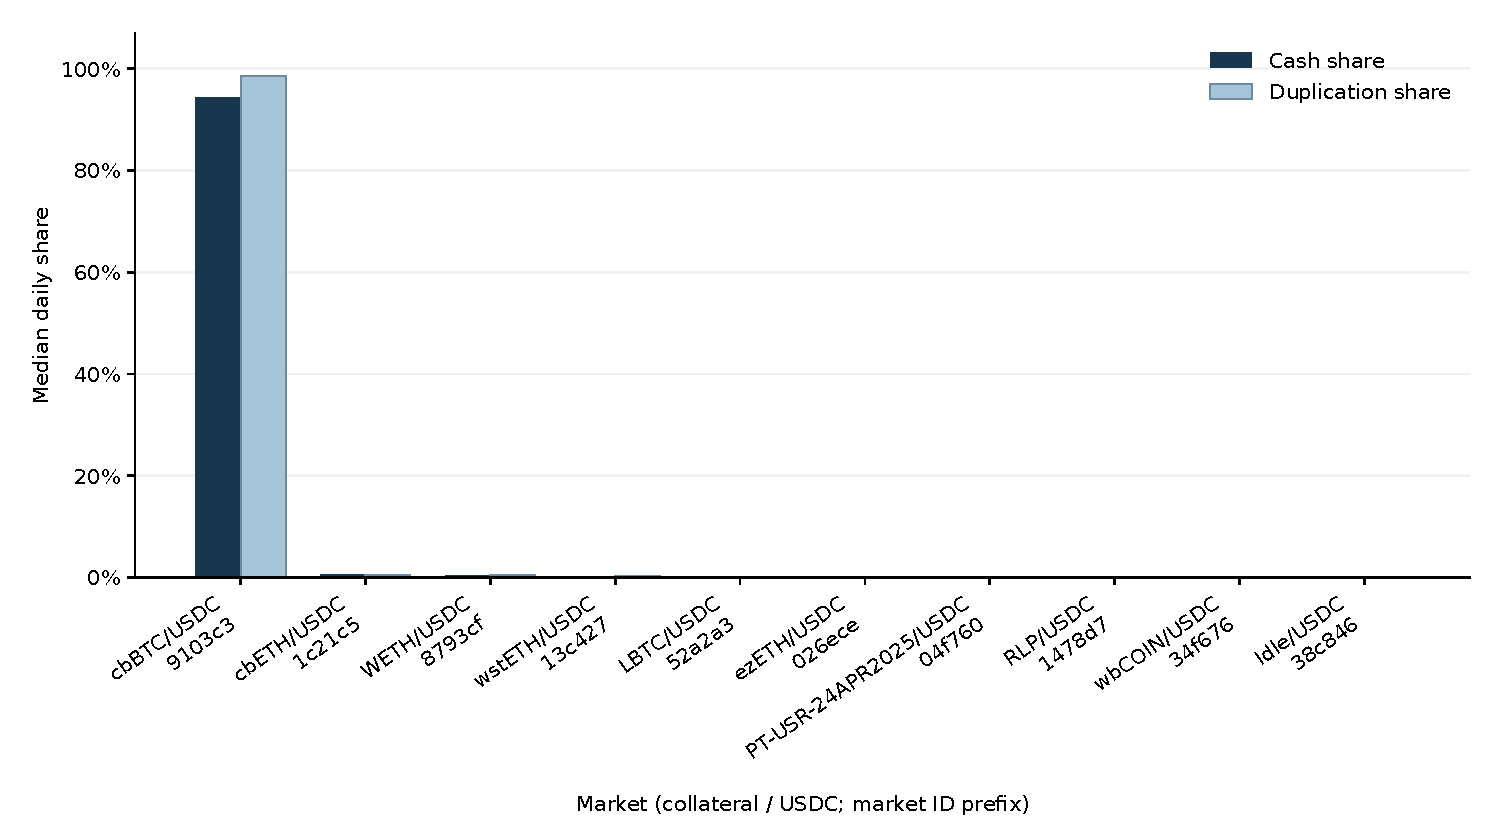
\includegraphics[width=\linewidth]{fig_market_shares.pdf}
\caption{Market cash shares and duplication shares}
\label{fig:marketshares}
\par\small\textit{Notes:} Each bar is the time median of a daily share in the fixed ten-vault sample. Markets are ranked by their median duplication share; market-ID order resolves ties. Market cash includes cash held in the fixed markets even on dates when the selected vaults have no position.\end{figure}

To assess dependence on vault composition, we enumerate all 1,023 nonempty subsets of the fixed ten-vault universe. For each subset size and date, we take the median duplication rate across subsets, and then take the time median. This statistic is 52.86\% for eight vaults, 56.86\% for nine vaults, and 58.19\% for all ten. The median daily increase between the ten- and eight-vault statistics is 4.63 percentage points. For eight-vault subsets, the corresponding median is 55.19\% when Spark is included and 31.72\% when it is excluded. The complete nine-vault portfolio excluding Spark has a median duplication rate of 34.47\%. Shared-cash overlap therefore extends beyond Spark, while its magnitude remains sensitive to portfolio composition.

\begin{figure}[htbp]\centering
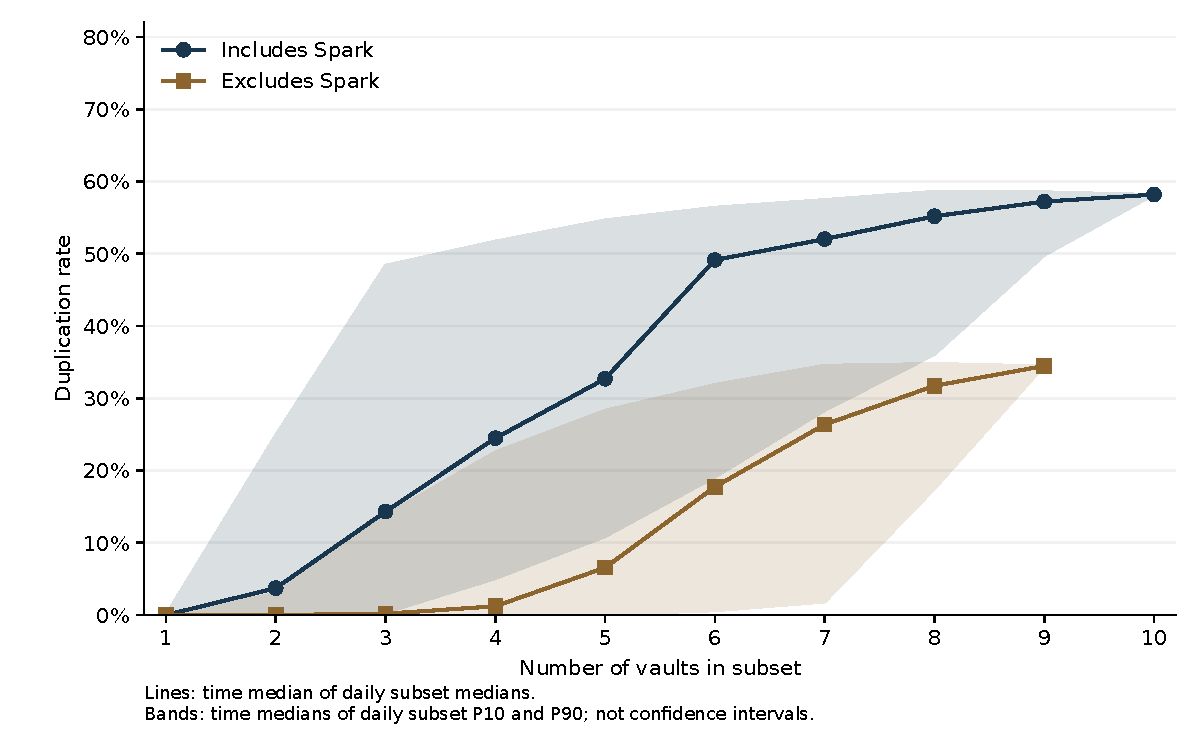
\includegraphics[width=.95\linewidth]{fig_k_curve.pdf}
\caption{Duplication rates across all vault subsets}
\label{fig:kcurve}
\par\small\textit{Notes:} Lines show the time median of daily within-group subset medians. Shaded bands show the time medians of daily within-group P10 and P90 values. The grouping indicates whether a subset includes Spark. Only subsets with positive standalone cash enter the daily distribution. No ten-vault subset excludes Spark. These bands describe subset dispersion.\end{figure}
